\section{Auswertung}
\label{sec:Auswertung}
\subsection{a)Messdaten}
\label{sec:messdaten}
Nachfolgend finden sich die aufgenommenen Messdaten ausgedrückt in SI-Einheiten. Zu den beiden Drücken $p_a$ und $p_b$ wurde jeweils $1 bar$ ($1\cdot10^5 Pa$) addiert. (vgl. \cite{Anleitung})
\begin{table}
  \centering
  \caption{Messdaten}

  \label{tab:Messdaten}
\begin{tabular}{cccccc}
\toprule
$\frac{t}{s}$ & $\frac{T_1}{K}$ & $\frac{T_2}{K}$& $\frac{p_b\cdot10^5}{Pa}$ & $\frac{p_a\cdot10^5}{Pa}$ & $\frac{P}{W}$ \\
\midrule
0.0 & 293.85 & 293.65 & 4.7 & 5.02 & 0.0 \\
60.0 & 293.95 & 293.65 & 6.7 & 4.22 & 119.0 \\
120.0 & 294.45 & 293.65 & 7.0 & 4.38 & 120.0 \\
180.0 & 295.75 & 293.65 & 7.1 & 4.43 & 123.0 \\
240.0 & 297.35 & 292.95 & 7.3 & 4.43 & 124.0 \\
300.0 & 298.65 & 292.05 & 7.5 & 4.39 & 123.0 \\
360.0 & 299.85 & 291.25 & 7.8 & 4.3 & 122.0 \\
420.0 & 300.55 & 290.35 & 8.0 & 4.21 & 121.0 \\
480.0 & 302.15 & 289.55 & 8.1 & 4.17 & 121.0 \\
540.0 & 303.25 & 288.85 & 8.3 & 4.02 & 120.0 \\
600.0 & 304.35 & 288.05 & 8.4 & 3.97 & 119.0 \\
660.0 & 305.25 & 287.35 & 8.7 & 3.88 & 119.0 \\
720.0 & 306.25 & 286.65 & 8.9 & 3.8 & 119.0 \\
780.0 & 307.15 & 286.05 & 9.0 & 3.77 & 119.0 \\
840.0 & 308.05 & 285.45 & 9.1 & 3.7 & 120.0 \\
900.0 & 308.95 & 284.95 & 9.3 & 3.63 & 120.0 \\
960.0 & 309.75 & 284.35 & 9.6 & 3.6 & 120.0 \\
1020.0 & 310.55 & 283.85 & 9.8 & 3.58 & 121.0 \\
1080.0 & 311.45 & 283.35 & 10.0 & 3.53 & 121.0 \\
1140.0 & 312.25 & 282.85 & 10.1 & 3.49 & 121.0 \\
1200.0 & 313.15 & 282.35 & 10.3 & 3.43 & 122.0 \\
1260.0 & 313.95 & 281.95 & 10.4 & 3.42 & 122.0 \\
1320.0 & 314.65 & 281.55 & 10.6 & 3.4 & 122.0 \\
1380.0 & 315.35 & 281.15 & 10.8 & 3.39 & 122.0 \\
1440.0 & 316.05 & 280.75 & 10.9 & 3.37 & 122.0 \\
1500.0 & 316.75 & 280.45 & 11.1 & 3.35 & 122.0 \\
1560.0 & 317.45 & 280.15 & 11.2 & 3.33 & 122.0 \\
1620.0 & 318.05 & 279.85 & 11.3 & 3.3 & 122.0 \\
1680.0 & 318.65 & 279.55 & 11.5 & 3.28 & 122.0 \\
1740.0 & 319.25 & 279.35 & 11.7 & 3.25 & 122.0 \\
1800.0 & 319.85 & 278.35 & 11.8 & 3.23 & 122.0 \\
1860.0 & 320.55 & 277.25 & 11.9 & 3.22 & 122.0 \\
1920.0 & 321.05 & 276.85 & 12.1 & 3.21 & 122.0 \\
1980.0 & 321.55 & 276.55 & 12.2 & 3.21 & 122.0 \\
2040.0 & 322.05 & 276.25 & 12.4 & 3.2 & 122.0 \\
2100.0 & 322.65 & 276.05 & 12.5 & 3.2 & 122.0 \\
2160.0 & 323.15 & 276.05 & 12.7 & 3.2 & 122.0 \\
\end{tabular}
\end{table}
\newpage
\subsection{b)Näherungsfunktion}
Eine nicht-lineare Ausgleichsrechnung mittels curvefit mithilfe der Näherungsfunktion
\begin{equation}
\label{eqn:naeherungsfunktion}
T(t)=\frac{At^\alpha}{1+Bt^\alpha}+C
\end{equation}

ergibt die folgenden Parameter
für $T_1(t)$\\

A= (0.006 \pm 0.001) $\frac{K}{s^\alpha}$ \\
$\alpha$= 1.197 \pm  0.036 \\
B= (0.00011 \pm 0.00002) $\frac{K}{s^\alpha}$\\
C= (293.2 \pm 0.2) $K$ \\

und für $T_2(t)$\\

A=(-0.001\pm 0.001)$\frac{K}{s^\alpha}$ \\
$\alpha$= 1.3 \pm 0.1 \\
B= (4.1 \pm 2.1) $\cdot 10^{-5}\frac{K}{s^\alpha}$\\
C= (294.3 \pm 0.3) $K$ \\

Im nachfolgenden Plot sind die Temperaturverläufe beider Reservoire mit einem zugehörigen Regressionsgraphen abgebildet.

\begin{figure}
  \centering
  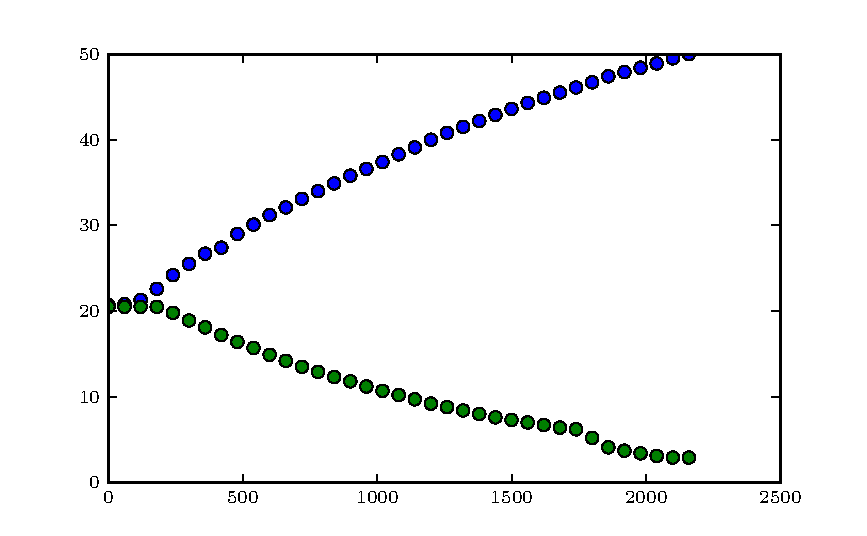
\includegraphics{build/plot.pdf}
  \caption{Temperaturverläufe beider Reservoire}
  \label{fig:temperaturverlauf}
\end{figure}


\subsection{c)}
Im Auswertungsteil c) sollen die Differentialquotienten $\frac{\symup{d}T_{1,2}}{\symup{d}t}$
für vier verschieden Temperaturen $T_i$ berechnet werden.

Nun gilt ja für die beiden Temperaturen $T_1$ und $T_2$ die Näherungsfunktion
\begin{equation}
	T_i(t) = \frac{A_i t^{\alpha_i}}{1 + B_i t^{\alpha_i}} + C_i
\end{equation}
Damit erhält man für den Differentialquotienten
\begin{equation}
	\frac{\symup{d}T_i}{\symup{d}t} = \frac{\alpha_i A_i t^{\alpha_i - 1}}{(1 + B_i t^{\alpha_i})^2}
\end{equation}
Es werden die vier Temperaturen zugehörig zu den Zeiten 300s, 600s, 900s und 1200s betrachtet.
Für $T_1$ ergeben sich die Werte
\begin{table}
\begin{tabular}{cccc}
	Zeit $t$ in s & Temperatur $T_1$ & $\frac{\symup{d}T_1}{\symup{d}t}$ & Fehler \\
	300 & 25,5 & 0,0191 & 0,0050 \\
	600 & 31,2 & 0,0175 & 0,0046 \\
	900 & 35,9 & 0,0151 & 0,0041 \\
	1200 & 40,0 & 0,0129 & 0,0036 \\
\end{tabular}
\end{table}

Für $T_2$ ergeben sich die Werte
\begin{table}
\begin{tabular}{cccc}
	Zeit $t$ in s & Temperatur $T_2$ & $\frac{\symup{d}T_2}{\symup{d}t}$ & Fehler \\
	300 & 18,9 & -0,0063 & 0,0063 \\
	600 & 14,9 & -0,0065 & 0,0066 \\
	900 & 11,9 & -0,0061 & 0,0062 \\
	1200 & 9,2 & -0,0055 & 0,0057 \\
\end{tabular}
\end{table}

$\sqrt{\frac{4 A^{2} a^{2} \sigma_{B}^{2} t^{2 a}}{\left(B t^{a} + 1\right)^{6}} t^{2 a - 2} + \frac{a^{2} \sigma_{A}^{2} t^{2 a - 2}}{\left(B t^{a} + 1\right)^{4}} + \sigma_{a}^{2} \left(- \frac{2 A B a t^{a} t^{a - 1}}{\left(B t^{a} + 1\right)^{3}} \log{\left (t \right )} + \frac{A a t^{a - 1}}{\left(B t^{a} + 1\right)^{2}} \log{\left (t \right )} + \frac{A t^{a - 1}}{\left(B t^{a} + 1\right)^{2}}\right)^{2}}$
\newpage


\subsection{d) Güteziffer der Wärmepumpe}

\subsection{e) Bestimmung des Massendurchsatz}
Zur Berechnung des Massendurchsatzes muss die Verdampfungswärme $L$ bestimmt werden.
Diese wird aus den Wertepaaren (p,T) und einer linearen Ausgleichsrechnung nach \eqref{eqn:ausgleichsgrade} bestimmt.

Die Verdampfungswärme ergibt sich dann nach $ L = −m \cdot R$, wobei $m$ die Steigung der Geraden und $R$ die allgemeine Gaskonstante ist.

Für $m$=(-2017 \pm 15)$K$ und $R$=(8.3144598 \pm 0.0000048) $\frac{J}{mol\cdot K}$ \cite{gas}
ergibt sich nach der Gauß’schen Fehlerfortpflanzung \eqref{eqn:fehlerfortpflanzung} der Fehler der Verdampungfswärme $L$.

$L$=(16770.3\pm 124.7)$\frac{J}{mol \cdot K}$


\begin{figure}
  \centering
  \includegraphics{build/ex_e.pdf}
  \caption{Plot der Verdampfungswärme}
  \label{fig:verdampfungswaerme}
\end{figure}


Der Massendurchsatz berechnet sich nun nach Gleichung \eqref{eqn:massendurchsatz}.
Da
\begin{equation}
	\frac{\symup{d}T_i}{\symup{d}t} = \frac{\alpha_i A_i t^{\alpha_i - 1}}{(1 + B_i t^{\alpha_i})^2}
\end{equation}

gilt, ergibt sich für den Massendurchsatz mit $m_W c_W=16727\frac{J}{K}$ \cite{eichler} und $m_k c_k=750\frac{J}{K}$ und  $L$=(16770.3\pm 124.7)$\frac{J}{mol \cdot K}$

\begin{table}
  \caption{Massendurchsatz}
  \begin{tabular}{ccc}
    \toprule
    Zeit $t$ in s & Massendurchsatz $\diff{m}{t} in \frac{mol}{s}$& $\diff{m}{t} in \frac{g}{s}$\\
    \midrule
300 & 0.018 \pm 0.005 &2.2 \pm 0.6\\
600 & 0.017 \pm 0.004 & 2.0 \pm 0.5\\
900 & 0.015 \pm 0.004 & 1.8 \pm 0.4\\
1200 & 0.0126 \pm 0.0031 & 1.5 \pm 0.4\\
    \end{tabular}
\end{table}
\subsection{f) Bestimmung der mechanischen Kompressorleistung}

Zur Bestimmung der mechanischen Kompressorleistung nach \eqref{eqn:kompressorleistung} muss zunächst die Dichte bestimmt werden.


damit ergibt sich die Kompressorleistung zu
\begin{table}
  \caption{}
  \label{}
  \begin{tabular} {ccc}
    Zeit $t$ in s & Dichte in& Kompressorleistung in\\
    \midrule
300 & 0.018 \pm 0.005 &21 \pm 6\\
600 & 0.017 \pm 0.004 & 22 \pm 6\\
900 & 0.015 \pm 0.004 & 21 \pm 5\\
1200 & 0.0126 \pm 0.0031 & 19 \pm 5\\

\end{tabular}
\end{table}
